\documentclass[12pt]{article}
 
\usepackage[T1]{fontenc}
\usepackage[polish]{babel}
\usepackage[utf8]{inputenc}
\usepackage{lmodern}
\usepackage{amsmath}
\usepackage{hyperref}
\usepackage{graphicx}
\usepackage{float}
%\usepackage[showframe,pass]{geometry}
\usepackage{caption}
\usepackage[linesnumbered,boxruled]{algorithm2e}
\usepackage[multiple]{footmisc}
\usepackage{subcaption}

\selectlanguage{polish}
 
\title{Algorytmy grafowe}
\author{Mateusz Bednarski (11794), Nikodem Hynek (117209)} 
\date{}
 
\begin{document}
\maketitle

\section{Wstęp}
Celem pracy jest implementacja dwóch podstawowych metod reprezentacji grafu. Przez listę następników oraz macierz sąsiedztwa. Dla każdej z tych reprezentacji zaimplementowano dwa algorytmy: przechodzenie w głąb i wszerz. Daje to w sumie cztery algorytmy:

\begin{itemize}
\item BFS list
\item DFS list
\item BFS matrix
\item DFS matrix
\end{itemize}

\section{Metodyka testów}
Algorytmy zostały przygotowane w języku Python (2.7.6), wersja 64-bit. Komputer na którym odbyły się pomiary:
8 GB RAM, Intel i5 3,1GHz pracujący pod kontrolą systemu Windows 8.1 (x64). Wykresy zostały wygenerowane
przy użyciu bibliotek \emph{matplotlib} oraz \emph{prettyplotlib} Sprawozdanie powstało przy użyciu systemu składu tekstu \LaTeX .
Wielkości próbek (n) dla każdego algorytmu to 11, 72, 143, 215, 286, 357, 429, 500, 571, 643, 714, 785, 857, 928 oraz 1000 elementów (liczb całkowitych nieujemnych). Każdy punkt wykresu pokazuje średnią ze 1000 pomiarów oraz odchylenie standardowe.

\section{Lista następników}
Reprezentacja grafu w postaci listy następników polega na utworzeniu słownika (tablicy asocjacyjnej/mapy) której kluczami są węzły a wartościami listy następników tychże węzłów.
\subsection{BFS}

\begin{algorithm}[H]
\KwData{
graph --- tablica asocjacyjna grafu \\
start --- wierzchołek startowy \\
path[] --- lista kolejno odwiedzonych wierzchołków
}
\Begin
{
stack $\leftarrow$ utwórz listę stack.append(start) \\
\While{start jest niepusty}
	{
		current $\leftarrow$ 	stack.pop()\\
		\If{$\neg$ current $\in$ path}
		{
		path.append(current)
		stack $\leftarrow$ graph[current] + stack
		} 
		
	}
	return path

	
}
\caption{BFS\textunderscore list}
\end{algorithm}	
Złożoność algorytmu wynosi $\mathcal{O}(|V| + |E|)$.


\subsection{DFS}
\begin{algorithm}[H]
\KwData{
graph --- tablica asocjacyjna grafu \\
start --- wierzchołek startowy \\
path[] --- lista kolejno odwiedzonych wierzchołków
}
\Begin
{
queue $\leftarrow$ utwórz kolejkę queue.enqueue(start) \\
\While{queue jest niepusta}
	{
		current $\leftarrow$ 	queue.dequeue()\\
		\If{$\neg$ current $\in$ path}
		{
		path.append(current)\\
		zakolejkuj wszystkich nieodwiedzonych następników.
		} 
		
	}
	return path

	
}
\caption{DFS\textunderscore list}
\end{algorithm}	
Złożoność algorytmu wynosi $\mathcal{O}(|V| + |E|)$.


\section{Macierz sąsiedztwa}
Implementacja w oparciu o macierz sąsiedztwa jest bardzo prosta. Tworzymy macierz o rozmiarze $n \times n$ i wypełniamy ją zerami. Teraz jeżeli istnieje łuk między węzłami $a$ i $b$ to ustawiamy matrix[a][b] = 1.

\subsection{DFS}
\begin{algorithm}[H]
\KwData{
n --- ilość węzłów\\
discovered[n] --- tablica typu bool zainicjowana wartością \emph{false} \\
v --- wierzchołek od którego zaczynamy przejście.
}
\Begin
{
	print(v) \\
	discovered[v] $\leftarrow$ \emph{true} \\
	\ForEach {w będącego sąsiadem v }
	{
		\If{$\neg$ discovered[w]}
		{
			DFS\textunderscore matrix(w)
		}
	}
}
\caption{DFS\textunderscore matrix}
\end{algorithm}	

Złożoność algorytmu wynosi $\mathcal{O}(|V| + |E|)$.
\subsection{BFS}
\begin{algorithm}[H]
\KwData{
n --- ilość węzłów\\
BLACK, GRAY, WHITE --- stałe \\
s --- wierzchołek od którego rozpoczyna się przechodzenie \\
color, dist, parent --- tablice $n$-wymiarowe
}
\Begin
{
	zainicjuj tablicę color wartością WHITE\\
	zainicjuj tablicę dist wartością $+\infty$\\
	zainicjuj tablicę color wartością \emph{null}\\
	color[s] $\leftarrow$ GRAY\\
	dist[s] $\leftarrow$ 0\\
	parent[s] $\leftarrow$ \emph{null} \\
	q $\leftarrow$ zainicjuj kolejkę \\
	q.enqueue(s) \\
	\While {q jest niepusta}
	{
		u $\leftarrow$ q.dequeue() \\
		\ForEach {v będącego sąsiadem u}
		{
			\If{color[v] = WHITE}
			{
				color[v] = GRAY\\
				dist[v] = dist[u] + 1 \\
				parent[v] = u
			}
		}
		color[u] $\leftarrow$ BLACK\\
		print(u)
	}
}
\caption{BFS\textunderscore matrix}
\end{algorithm}	

Złożoność algorytmu wynosi $\mathcal{O}(|V| + |E|)$.

\section{Testy}
\begin{figure}[H]
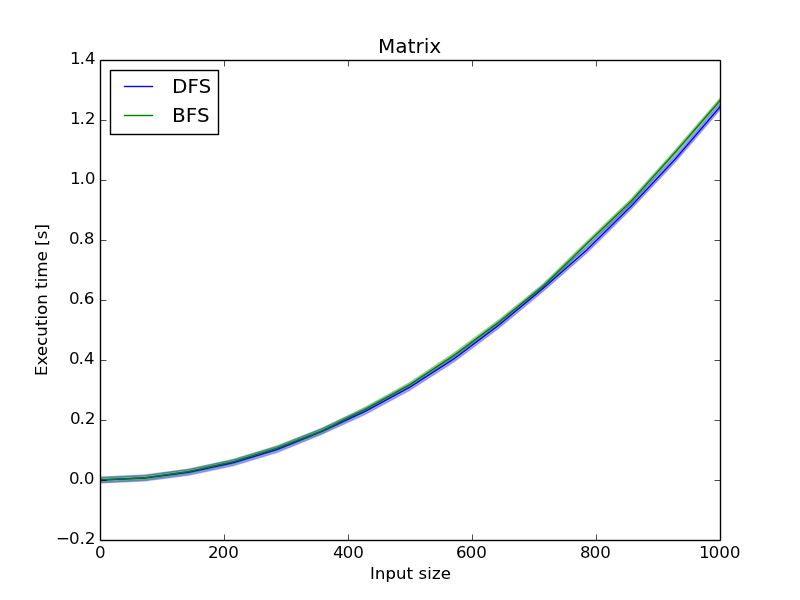
\includegraphics[width=\textwidth,keepaspectratio=true]{matrix/matrix.png}
\caption{Wykres $t(n)$ dla algorytmów \emph{BFS\textunderscore matrix} i \emph{BFS \textunderscore matrix}. Widać że zachowują się praktycznie tak samo.}
\end{figure}
\begin{figure}[H]
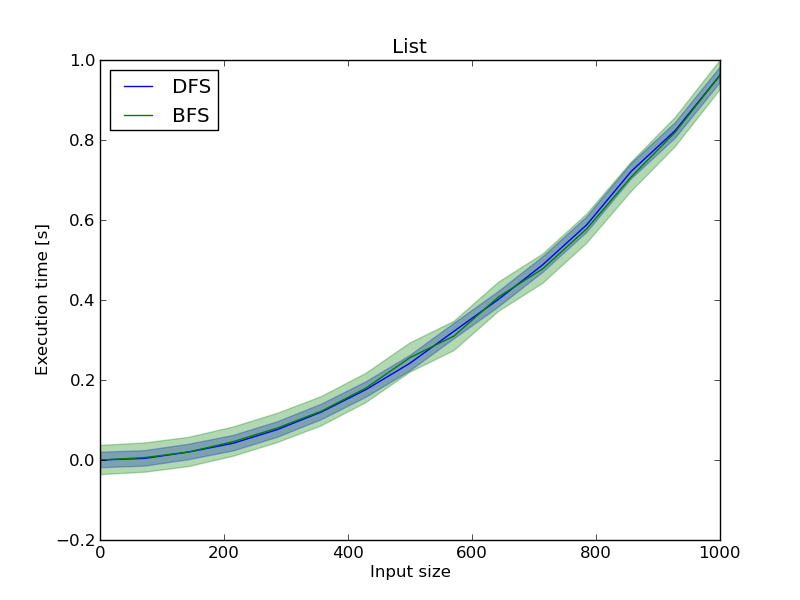
\includegraphics[width=\textwidth,keepaspectratio=true]{matrix/list.png}
\caption{Wykres $t(n)$ dla algorytmów \emph{BFS\textunderscore list} i \emph{BFS \textunderscore list}. Złożoność jest taka sama.}
\end{figure}

\section{Bonus}
\begin{quote}
Zadanie bonusowe polegało na zaproponowaniu algorytmu znajdowania ścieżek. Postawiony problem brzmi następująco: 
Posiadasz plan pewnego muzeum – jest ono w formie kwadratu podzielonego na n * n równych
pomieszczeń ( n – dowolna liczba całkowita). W każdym pomieszczeniu możliwa jest tylko jedna z
trzech następujących sytuacji: zwiedzający oglądają znajdujące się tam dzieła sztuki, w
pomieszczeniu znajduje się strażnik lub pomieszczenie jest puste. Twoim zadaniem jest znaleźć
ścieżkę z pomieszczenia A do pomieszczenia B (o ile to możliwe) taką, że składa się ona z pustych
pomieszczeń możliwe najbardziej odległych od strażników. Przyjmij, że liczba strażników wynosi
m, natomiast przechodzenie z pomieszczenia do pomieszczenia możliwe jest tylko horyzontalnie i
wertykalnie. Dodatkowo możesz przyjść że punkt A jest jednym z pomieszczeń przy brzegu
budynku (wyjście z muzeum), wówczas punkt B może oznaczać pomieszczenie z najbardziej
wartościowym dziełem sztuki. Przyjmujemy, że pomieszczenia A i B są puste.
\end{quote}
Kolejne sekcje szczegółowo omawiają sposób rozwiązania opracowany przez autorów.
\subsection{Dane wejściowe}
Algorytm przyjmuje następujące parametry wejściowe:
\begin{description}
\item[n] Wielkość mapy (bok kwadratu)
\item[m] Procent strażników
\item[vp] Procent pokoi zajętych przez zwiedzających
\item[startPos] Miejsce startowe
\item[treasurePos] Lokacja najbardziej wartościowego łupu
\item[guard\textunderscore range] Zasięg strażnika

\end{description}
\subsubsection{Zasięg strażnika}
Ostatni parametr wejściowy wymaga szerszego komentarza. W przyjętym rozwiązaniu każdy strażnik roztacza wokół siebie pole wektorowe. Jego wyższa wartość oznacza większe prawdopodobieństwo zauważenia intruza. Zasięg oznacza maksymalną odległość (w metryce taksówkowej) do której sięga generowane przez niego pole. Sposób generowania pola zostanie omówiony przy algorytmach pomocniczych.

\subsection{Sposób reprezentacji danych}
Problem jest reprezentowany przez macierz o rozmiarze $n \times n$. Każda komórka zawiera liczbę całkowitą kodującą jej stan. Możliwe wartości to:
\begin{description}
\item[-5] Przez pole przebiega znaleziona ścieżka
\item[-4] Pole zawierające łup
\item[-3] Pole startowe
\item[-2] Pole zawierające strażnika
\item[-1] Pole zawierające zwiedzającego
\item[0+] Pole puste, wartość oznacza ,,koszt'' przejścia (tym większy im bliżej są strażnicy)
\end{description}

Wraz z algorytmem powstał program rysujący mapę.
\begin{figure}
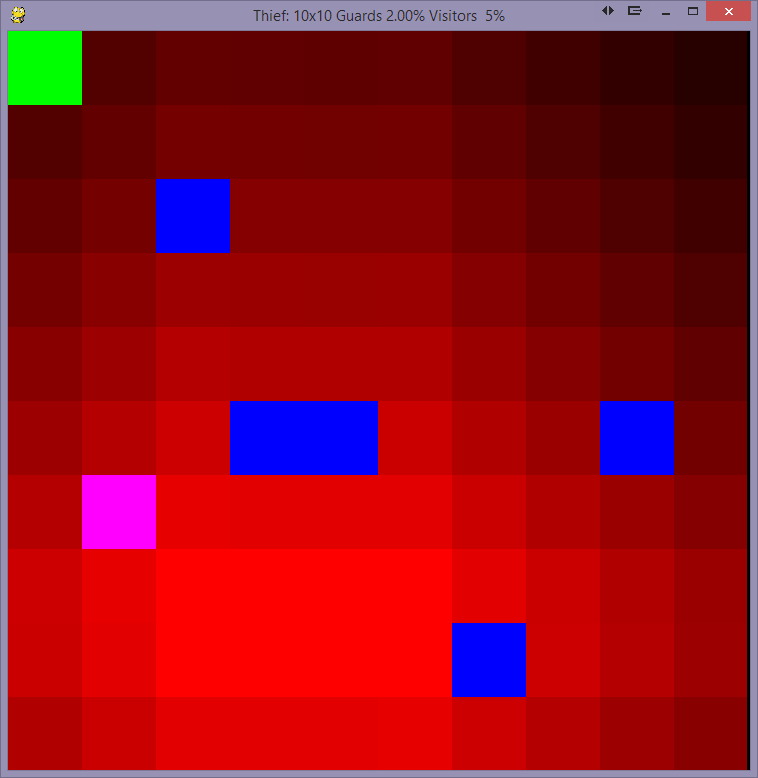
\includegraphics[width=\textwidth,keepaspectratio=true]{Clipboard01.png} 
\caption[]{Mapa wygenerowana dla parametrów $n=10$, $m=2\% $,\\\hspace{\textwidth} $\text{vp}=10\%$, $\text{startPos}=[0,0]$, $\text{treasurePos}=[6,1]$, $\text{guard range}=20$ \\\hspace{\textwidth} Kolor zielony oznacza miejsce startowe. Różowy --- łup, niebieski --- zwiedzającego. Nasycenie czerwonego --- wartość pola skalarnego. Kolory są skalowane liniowo tak aby \#FF0000 oznaczał maksymalną wartość pola na całej mapie a \#000000 wartość zerową. Wartość \#FF0000 oznacza również strażnika. }
\end{figure}

\subsection{Pole generowane przez strażnika}
Każdy strażnik roztacza wokół siebie pole wektorowe. Do generowania zastosowano dwie funkcje, z czego jedna z nich została ostatecznie użyta\footnote{ Drugą funkcją jest \emph{linear\textunderscore cost} w pliku \emph{museum.py}}.

\begin{figure}[!ht, caption=xd]
\centering
\[
 J(x) =
  \begin{cases}
   0 & \text{dla } x = 0\, \vee x > C_1\\
   \frac{C_1^2}{C_2} (x-C_1)^2 + 1       &  \text{dla } x \in (0, C_1)  
  \end{cases}
\]
\caption*{Kwadratowa funkcja kosztu. Argumentem jest odległość pola od strażnika. $C_1$ oraz $C_2$ oznaczają odpowiednio zasięg strażnika oraz bazowy koszt przejścia (na polu ze strażnikiem). W praktyce wielkość $C_2$ współczynnika jest nieistotna, byłoby inaczej gdyby istniały klasy strażników o różnej wartości np. strażnik z bronią miał by tą wartość większą, niż ochroniarz z grupą inwalidzką)}
\end{figure}

\begin{figure}[h]
\centering
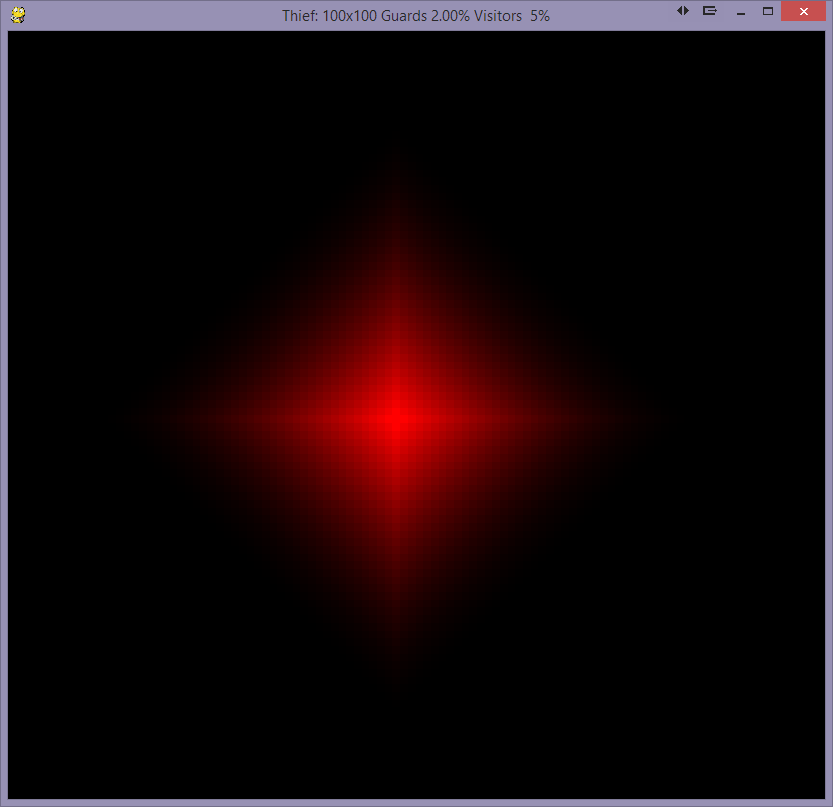
\includegraphics[scale=0.25,keepaspectratio=true]{Clipboard02.png} 
\caption{Pole generowane przez pojedynczego strażnika.}
\end{figure}

\subsection{Algorytmy pomocnicze}
Na potrzeby głównego algorytmu powstało kilka mniejszych (pomocniczych).
\subsubsection{Odległość w sensie metryki taksówkowej}

\begin{algorithm}[H]
\KwData{$\vec{a}$, $\vec{b}$ --- współrzędne dwóch punktów}
\KwResult {Odległość}
\Begin
{
\Return $|x_a - x_b| + |y_a - y_b|$
}
\caption{distance}
\end{algorithm}

Złożoność alorytmu wynosi $\mathcal{O}(1)$.

\subsubsection{Dodanie pola pochodzącego od nowego strażnika}


\begin{algorithm}[H]
\KwData{ pos --- współrzędne strażnika, n --- rozmiar mapy}
\KwResult {Odległość}
\tcc{gr oznacza zasięg strażnika}
\Begin
{
	\ForEach{ pos.y - gr < y < pos.y + gr  } 
	{
		\ForEach{ pos.x - gr < x < pos.x + gr  } 
		{
			\If {$0 \leq x \leq n\, \wedge 0 \leq y \leq n\, $ x}
			{
			 	\If {$[x, y]$ nie jest zajęty}
			 	{
			 		$\text{cost} \leftarrow J(\text{dist}(pos, [y,x])$ \\
			 		matrix[y][x] += cost
			 	}
			}
		}
	}
}

\caption{append\textunderscore field}
\end{algorithm}
Złożoność wynosi $\mathcal{O}(n^2)$ gdzie $n$ jest zasięgiem strażnika.

\subsubsection{Rozmieść strażników}
\begin{algorithm}[H]
\KwData{n --- ilość strażników}
\tcc{is\textunderscore prohibited sprawdza czy na danym polu można umieścić strażnika tj. czy nie zawiera ono już innego obiektu}
\Begin
{
	put $\leftarrow$ 0 \\
	\While{put < n}
	{
		pos $\leftarrow$ wylosuj pozycję na planszy \\
		\If {$\neg \text{is\textunderscore prohibited}(\text{pos}) $}
		{
			ustaw pole \emph{pos} w macierzy na -2 (strażnik) \\
			append\textunderscore field(pos) \\
			put += 1
		}
	}
	
}
\caption{put\textunderscore guards}
\end{algorithm}

Algorytm dba o to aby zostało rozmieszczone \emph{dokładnie} $n$ strażników. Jeśli wylosowane pole jest już zajęte, próbuje dalej. W szczególnym przypadku algorytm nigdy się nie kończy (strażników do rozmieszenia jest więcej niż wolnych pól). Złożoność określamy jako $\mathcal{O}(n^3)$ (ze względu na 7 linię) chociaż dla małych plansz z dużą ilością strażników będzie ona rosła ze względu na ponawianie losowań. Ustawianie zwiedzających jest analogicznie, jedyną różnicą jest wstawianie $-1$ w miejsce $-2$ więc nie jest ono tutaj prezentowane.

\subsection{Generowanie mapy}
Algorytm generowania mapy należy zasadniczo do algorytmów pomocniczych, jednak ze względu na swoją wagę zostanie omówiony osobno.

\begin{algorithm}[H]
\KwData{
n --- Wielkość mapy (bok kwadratu) \\
m --- Procent strażników \\
vp --- Procent pokoi zajętych przez zwiedzających \\
sp --- Miejsce startowe \\
tp --- Lokacja najbardziej wartościowego łupu \\
gr --- Zasięg strażnika
}
\Begin
{
	zainicjuj macierz \emph{matrix} o rozmiarze $n\times n$ \\
	matrix[$s_p$] $\leftarrow$ -3 \\
	matrix[$t_p$] $\leftarrow$ -4 \\
	gc $\leftarrow n^2 \cdot m \div 100 $ \\
	vc $\leftarrow n^2 \cdot vp \div 100 $ \\
	put\textunderscore guards($g_c$) \\
	put\textunderscore visitors($v_c$)	
}
\caption{Konstruktor klasy \emph{Museum}}
\end{algorithm}

Algorytm jest bardzo prosty i nie wymaga specjalnego komentarza. Przyjrzyjmy się jednak jego złożoności. W tabeli przedstawiono złożoność instrukcji w kolejnych liniach:
\begin{tabular}{|c|c|c|c|c|c|c|}
\hline 
2 & 3 & 4 & 5 & 6 & 7 & 8 \\ 
\hline 
$\mathcal{O}(1)$ & $\mathcal{O}(1)$ & $\mathcal{O}(1)$ & $\mathcal{O}(1)$ & $\mathcal{O}(1)$ & $\mathcal{O}(g_c \cdot g_r^2)$ & $\mathcal{O}(\text{vc})$ \\ 
\hline 
\end{tabular} 
Daje to $\mathcal{O}(5 + g_c \cdot g_r^2 + v_c )$. Następnie 
\begin{equation*}
\mathcal{O} \left(
5 + n^2 \cdot m \cdot g_r^2 + n^2 \cdot v_p
 \right)
\end{equation*}
Przy racjonalnym założeniu, że $m \approx \text{vp}$
\begin{equation*}
\mathcal{O} \left(
5 + n^2 \cdot m \cdot g_r^2 + n^2 \cdot v_p
\right)
\end{equation*}
Ostatecznie
\begin{equation*}
\mathcal{O}\left(n^2( m g_r^2 + v_p ) \right)
\end{equation*}

Wyliczona złożoność jest dość wysoka. Jest to spowodowane doliczaniem wartości generowanych przez pole dookoła strażnika. Jak się jednak później okaże się że taka reprezentacja danych jest efektywna przy wyszukiwaniu drogi.


\subsection{Znajdowanie drogi}

Zaproponowany algorytm znajdowania drogi został w całości wymyślony przez autorów. Został zaimplementowany w dwóch wersjach: normalnej i ,,nie niszczącej''. Druga wersja nie zaznacza znalezionej drogi i została przygotowana na potrzeby pomiarów.

Algorytm pracuje w dwóch fazach, które zostaną omówione osobno.

\subsubsection{Budowanie macierzy kosztu}
Faza pierwsza polega na przejściu całej mapy i wpisaniu w każde pole minimalnego kosztu przejścia do niego. Zaczynamy od pola startowego i wszędzie dookoła wrzucamy koszt obecnego pola + 1 + koszt pola sąsiedniego. Dodawanie jedynki sprawia że spośród kilku ścieżek o tym samym sumarycznym koszcie algorytm preferuje krótszą. Jako że do jednego pola można dojść z kilku stron, algorytm wybiera tą o najniższym koszcie.

Faza kończy się po dotarciu do łupu. W takim przypadku część tablicy \emph{hard} może pozostać nieuzupełniona. Nie jest to problemem ponieważ wszystkie koszty są dodatnie, więc wiadomo już że nie da się znaleźć ,,tańszej'' ścieżki.

Złożoność algorytmu szacujemy na $\mathcal{O}(n^2)$
\begin{algorithm}[p]
\KwData{
n --- Wielkość mapy (bok kwadratu) \\
sp --- Miejsce startowe \\
matrix --- wygenerowana plansza}
\KwResult {hard --- macierz kosztów osiągnięcia każdego pola} 
\tcc{ is\textunderscore way - czy przez pole można przejść}
\Begin
{
	hard $\leftarrow$ zainicjuj macierz $n \times n$ wartością $+\infty$ \\
	visited $\leftarrow$ zainicjuj macierz $n \times n$ wartością 
\emph{false} \\
	q $\leftarrow$ utwórz kolejkę \\
	q.enqueue(sp) \\
	\While{ q jest niepusta }
	{
		curr $\leftarrow$ q.dequeue()\\
		visited[curr] $\leftarrow$ \emph{true}\\
		\If {matrix[curr] = -4} 
		{
			\tcc {Znaleziono łup - przeszliśmy wystarczająco dużo}
			\Return hard
		}
		\ForEach{nb $\in$ pola\textunderscore sąsiednie\textunderscore do \textunderscore curr}
		{
			\If { $\neg$ is\textunderscore way(nb) $\vee$ visited[nb] }
			{
				\textbf{continue} 
			}
			newCost $\leftarrow$ 1 + hard[curr] + matrix[nb] \\
			oldCost $\leftarrow$ hard[nb] \\
			hard[nb] = min(newCost, oldCost) \\
			\If{nb $\notin$ q}
			{
				q.enqueue(nb)
			}
		}
		visited[curr] $\leftarrow$ \emph{true}
	}
	
	
}
\caption{steal (I)}
\end{algorithm}
\begin{figure}[H]
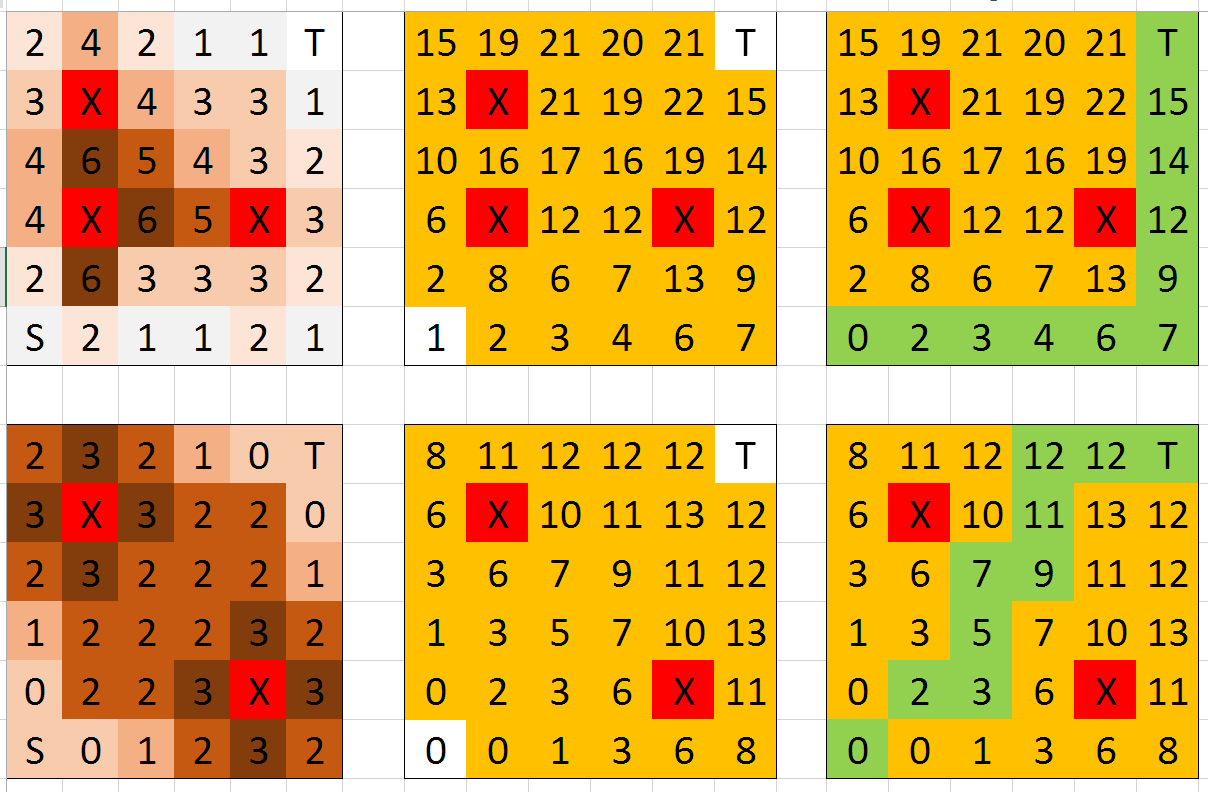
\includegraphics[width=\textwidth,keepaspectratio=true]{Capture.png}
\caption{
Macierz z danymi i macierze kosztu dla dwóch przykładowych danych.
Z lewej widać zawartość macierzy \emph{matrix} z zawartymi wartościami pola skalarnego. Macierz w środku prezentuje \emph{hard} (bez uwzględnienia dodatkowych jedynek). Widać, że im dalej od punktu startowego koszt dotarcia na pole rośnie. Macierze z prawej są również reprezentacją \emph{hard} ale z zaznaczonymi znalezionymi ścieżkami.
}
\end{figure}	

	
\subsubsection{Właściwe znajdowanie drogi}	
Mając w ten sposób przygotowaną macierz kosztu, znalezienie optymalnej drogi jest bardzo proste.

Zaczynamy w miejscu gdzie znajduje się łup. Następnie przechodzimy na sąsiednie pole o najmniejszym koszcie i oznaczamy je jako drogę \footnote{Istnieje jeszcze druga wersja algorytmu \emph{no\textunderscore destroy} która pomija ten krok - pozwala to na wielokrotne użycie tej samej macierzy w testach, bez konieczności generowania jej od nowa.}. Algorytm postępuje aż natrafi na jeden z dwóch przypadków:
\begin{enumerate}
\item Nie ma pola na które można przejść - oznacza to brak drogi między punktem startowym a eksponatem
\item dotarcie do punktu startowego - oznacza to osiągnięcie celu
\end{enumerate}

Złożoność szacujemy na $\mathcal{O}(n)$.
	


\begin{algorithm}[H]
\KwData{
n --- Wielkość mapy (bok kwadratu) \\
sp --- Miejsce startowe \\
matrix --- wygenerowana plansza \\
target --- lokacja łupu \\
hard --- macierz kosztu przejścia
}
\KwResult {hard --- macierz kosztów osiągnięcia każdego pola} 
\tcc{ is\textunderscore way - czy przez pole można przejść}
\Begin
{
	visited $\leftarrow$ zainicjuj macierz $n \times n$ wartością $0$\\
	iter $\leftarrow$ target \\
	\While { true }
	{
		\If{iterator = null}
		{ 
		 print ,,No Way!'' \\
		 \textbf{break}
		}
		\If{iterator = sp}
		{ \textbf{break}}		
		visited[iter] $\leftarrow$ \emph{true}\\
		matrix[iter] $\leftarrow$ -5 \tcc*{Oznacz jako drogę}
		local\textunderscore minima	$\leftarrow +\infty$\\
		next\textunderscore way $\leftarrow$ null \\
		\ForEach {nb $\in$ pola\textunderscore sąsiednie\textunderscore do $\wedge$ is\textunderscore way(nb)}
		{
			val $\leftarrow$ hard[nb]\\
			\If{val < local\textunderscore minima}
			{
				local\textunderscore minima $\leftarrow$ val\\
				next\textunderscore way $\leftarrow$ nb
			}
		}
		iterator $\leftarrow$ next\textunderscore way
		
	}
	
 }
\caption{steal (II)}
\end{algorithm}	

\subsection{Analiza}
\begin{figure}[H]
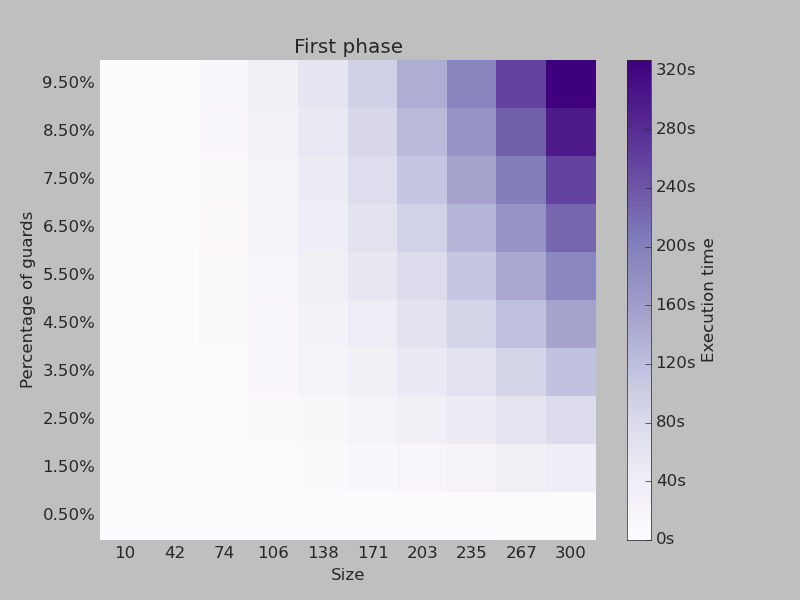
\includegraphics[width=\textwidth,keepaspectratio=true]{Thief/creations.png}
\caption{
Wykres utworzony dla pierwszej części algorytmu. Widać, że im większa gęstość strażników oraz wielkość mapy tym dłuższy czas generowania. Wpływ czynnika $g_r$ i $n$ są bardzo podobne, zgodnie z teoretycznymi przewidywaniami.}
\end{figure}	
\begin{figure}[H]
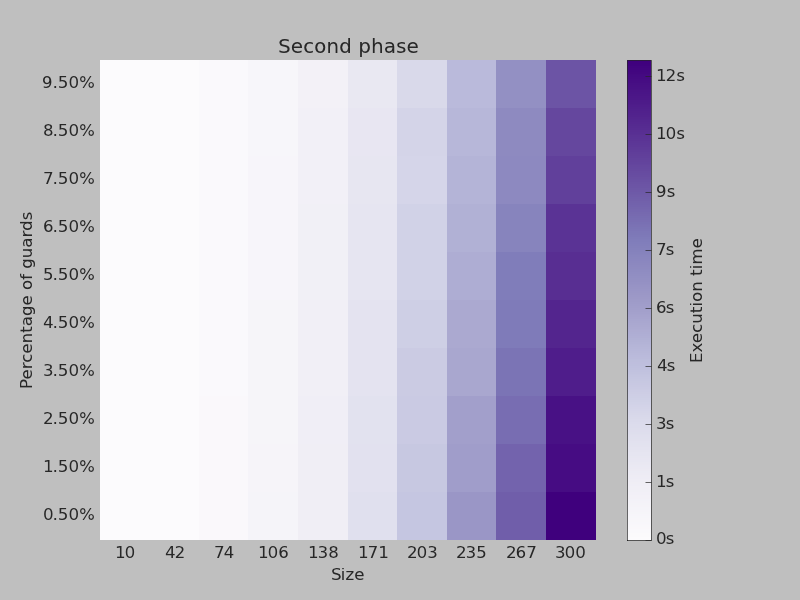
\includegraphics[width=\textwidth,keepaspectratio=true]{Thief/going.png}
\caption{
Wykres utworzony dla drugiej części algorytmu. Decydująca jest tutaj wielkość mapy (co również zgadza się z teorią). Wpływ ilości strażników jest niewielki i co ciekawe im jest ich więcej tym szybciej działa algorytm (przeciwnie niż w pierwszej fazie).
}
\end{figure}	
\begin{figure}[H]
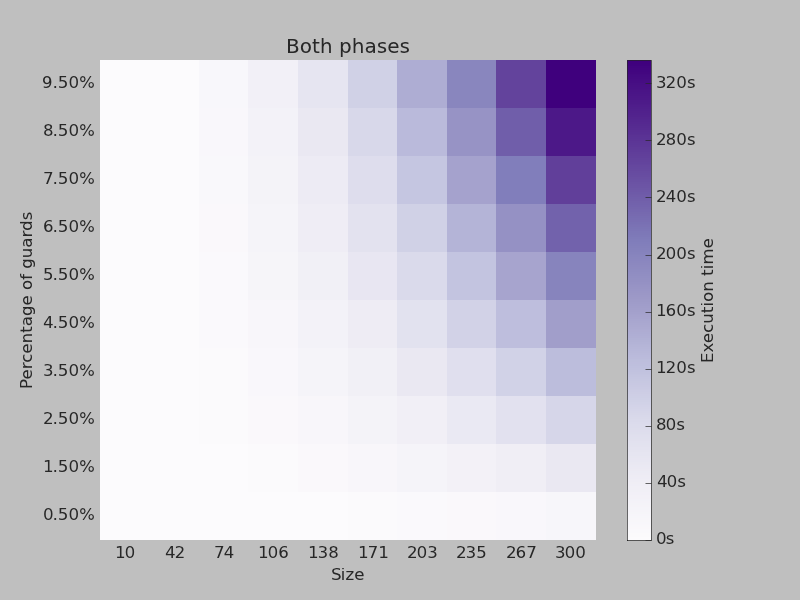
\includegraphics[width=\textwidth,keepaspectratio=true]{Thief/combined.png}
\caption{
Nałożone czasy wykonania obu faz. Jest on całkowicie zdominowany przez pierwszą fazę.
}
\end{figure}	

\subsection{Podsumowanie}
Autorzy początkowo rozważali użycie jednego ze znanych algorytmów ~m.~in. \emph{Floyda---Warshalla}, \emph{Dijkstry} oraz \emph{A*}. Ostatecznie uznali że realizacja własnego pomysłu będzie bardziej wartościowa niż rozwiązanie tego problemu tak samo po raz kolejny. Ponadto przejście przez cały proces od wymyślenia do zaimplementowania i przetestowania ma większą wartość edukacyjną.

Cały kod jest dostępny w serwisie Github - \url{https://github.com/Xevaquor/AiSD-Graph}

Algorytm łatwo da się rozszerzyć o dynamiczne przesuwanie strażników, jednakże nie wystarczyło na to czasu.

\begin{figure}
\begin{subfigure}[]{0.5\textwidth}
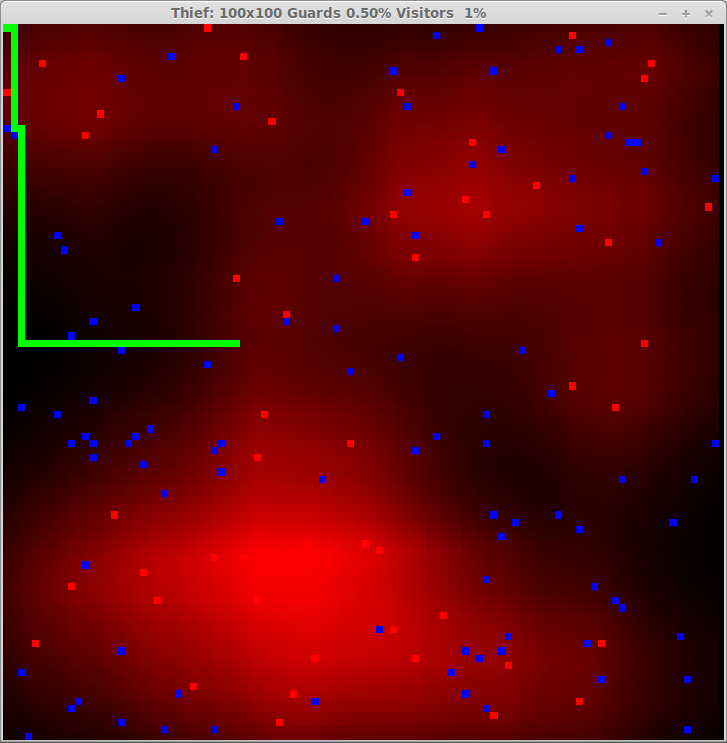
\includegraphics[width=\textwidth,keepaspectratio=true]{demo1.png}
\end{subfigure}
\begin{subfigure}[]{0.5\textwidth}
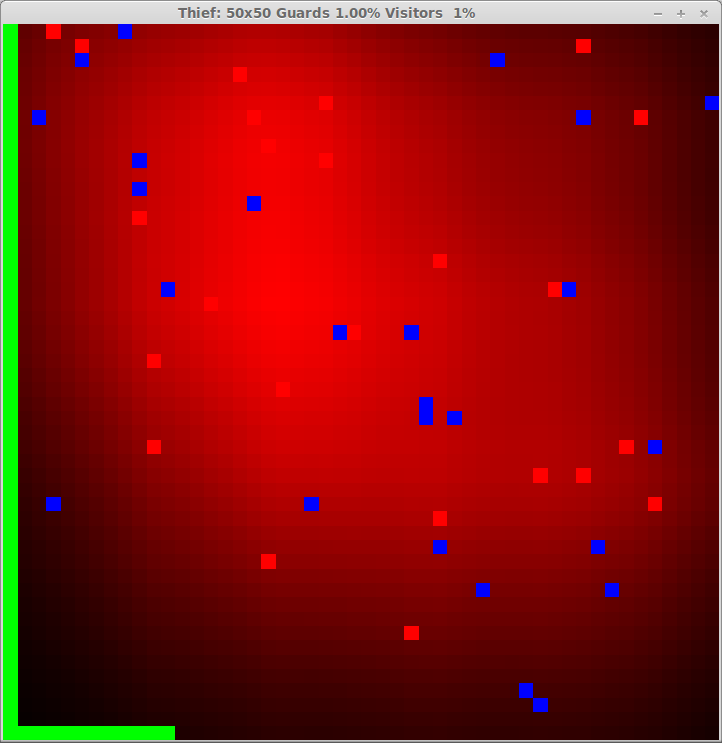
\includegraphics[width=\textwidth,keepaspectratio=true]{demo2.png}
\end{subfigure}
\begin{subfigure}[]{0.5\textwidth}
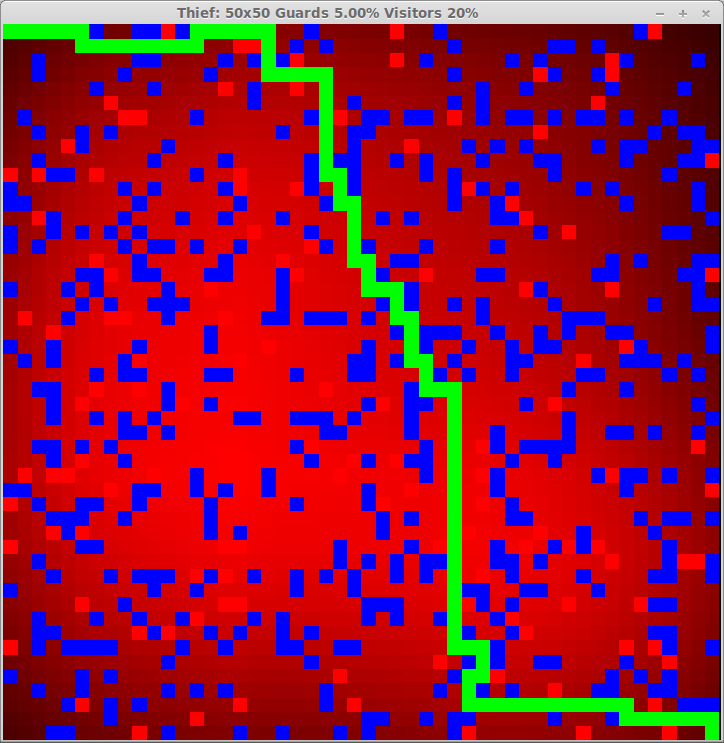
\includegraphics[width=\textwidth,keepaspectratio=true]{demo3.png}
\end{subfigure}
\begin{subfigure}[]{0.5\textwidth}
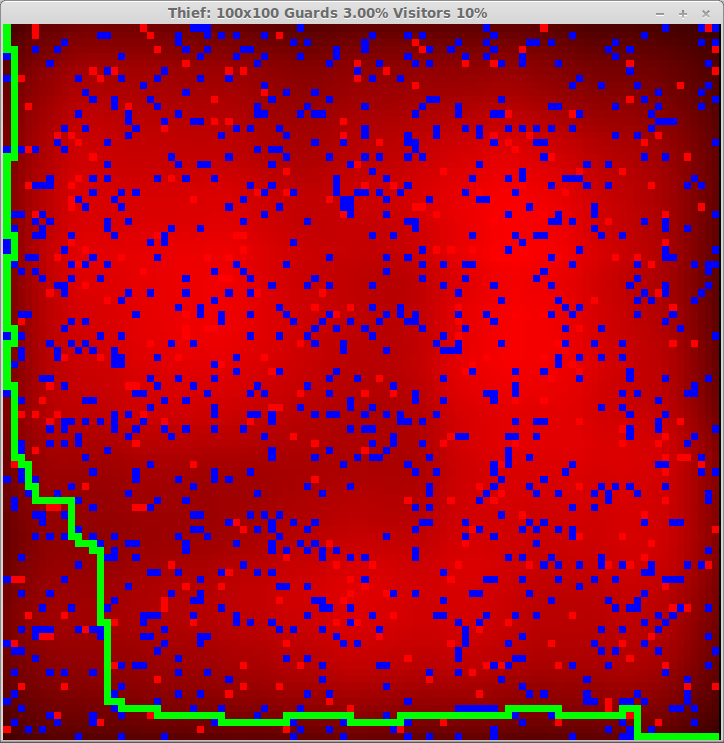
\includegraphics[width=\textwidth,keepaspectratio=true]{demo4.png}
\end{subfigure}
\caption{Przykładowe wyniki działania algorytmu.}
\end{figure}

\end{document}